% id: 20-08
% book: 100발100중 3-2 기말 · 01 3-2 기말(원의 성질·통계·부록)
% section: 실전 문제 2회
% figure: crop:fig-20-08.png
% answer: ②
% answer_source: 답지(빠른정답)
% variant_level: 0 (원본 전사)
% 이 파일은 build.mjs 가 items.json 에서 만든다. 고칠 때는 items.json 을 고친다.
\smash{\raisebox{1.5mm}{\dmkichul{100발100중 3-2 기말 20쪽 08번}}}
\noindent\begin{minipage}[t]{0.58\linewidth}\vspace{0pt}\raggedright 그림과 같이 무대의 길이가 $30\mkern3mu \mathrm{m}$인 원 모양의 공연장이 있다. 공연장의 $\pt{A}$지점에서 무대의 양 끝 $\pt{B}$, $\pt{C}$지점을 바라본 각의 크기가 $45^\circ$일 때, 이 공연장의 반지름의 길이는?\end{minipage}\hfill\begin{minipage}[t]{0.4\linewidth}\vspace{0pt}\centering 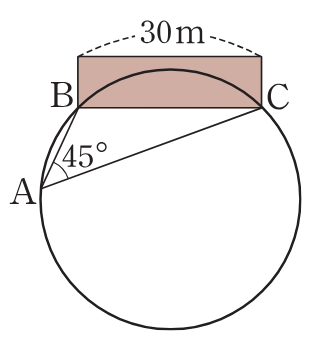
\includegraphics[width=74.0pt]{figures/fig-20-08.png}\end{minipage}\par
\begin{choices32}{\rule[-3ex]{0pt}{8ex}$15\mkern3mu \mathrm{m}$}{\rule[-3ex]{0pt}{8ex}$15\sqrt{2}\mkern3mu \mathrm{m}$}{\rule[-3ex]{0pt}{8ex}$15\sqrt{3}\mkern3mu \mathrm{m}$}{\rule[-3ex]{0pt}{8ex}$30\sqrt{2}\mkern3mu \mathrm{m}$}{\rule[-3ex]{0pt}{8ex}$30\sqrt{3}\mkern3mu \mathrm{m}$}\end{choices32}
